\documentclass[a4paper,12pt]{article}
\usepackage[english]{babel}
\usepackage{graphicx}
\usepackage{tikz}
\usepackage{wrapfig}
\usepackage{array}
\usepackage{color} 
\usepackage{hyperref}
\usepackage{enumitem}
\usepackage[normalem]{ulem}
\usepackage[font=small,labelfont=bf]{caption}
\usepackage{tcolorbox}
\hypersetup{
    colorlinks,
    citecolor=black,
    filecolor=black,
    linkcolor=black,
    urlcolor=black
}
\usepackage{changepage}
\addto{\captionsenglish}{\renewcommand{\refname}{}}

\begin{document}

\title{%
  Group Project Part 3 - ElasticSearch \\
  \large of Systems and Methods for Big
    and Unstructured Data Course \\(SMBUD)\\
    held by\\ Brambilla Marco\\ Tocchetti Andrea \\
  \vspace{5mm}
  \Large \textbf{Group 14}}
\author{Banfi Federico\\
  \texttt{10581441}
  \and
  Carotenuto Alessandro\\
  \texttt{10803080}
  \and
  Donati Riccardo\\
  \texttt{10669618}
  \and
  Mornatta Davide\\
  \texttt{10657647}
  \and
  Zancani Lea\\
  \texttt{10608972}}
\date{Academic year 2021/2022}
\maketitle
\begin{center}
  \includegraphics[width=4cm]{polilogo.png}\\
\end{center}
\newpage
\tableofcontents
\newpage
\section{Problem Specification}
\paragraph{}During the sanitary emergency due to the Covid-19 pandemic, many programs and applications developed thanks to the use of Big Data proved to be particularly effective in different settings and scenarios, such as the hospital administration, the hospitalizations organization or the analysis of data relating to various clinical cases. Among the various areas that have been supported by these technologies there is also that which concerns the tracking of populations belonging to a given geographical area and the collection of all information regarding the tests carried out and the vaccination status. \par
Our project aims to create an information system suitable for this specific use case and to do this it is necessary to design a database that allows us to store large amounts of data derived from heterogeneous sources and to carry out targeted queries useful for different purposes. The NOSQL document-based approach, known for being based on managing data saved in JSON-like documents, is the optimal one in this case and MongoDB is the open source database management software that is best suited to accomplish this task thanks to the considerable scalability guaranteed by the automatic data sharding and ease of use thanks to the dynamic schemes developed starting from the archived documents.
\section{Hypotheses}
\paragraph{} During the design phase,some considerations were made regarding how to structure and implement the database to obtain a solution that was effective and performing but at the same time consistent with the real current scenarios. First of all, two types of documents have been created: Certification and AuthorizedBody; the first represents a sort of ”medical chart” containing the following fundamental information for each individual:
  \begin{enumerate}[noitemsep]
    \item list of tests she/he has undergone,
    \item list of vaccine doses that have been administered,
    \item personal details (such as name, surname, date of birth, etc.),
    \item one or more emergency contacts to call in case of need.
   \end{enumerate}
Within the documents stored in the database for each of these four fields, subfields have been provided (as shown in the \texttt{"jsonSchema.json"} file into the \texttt{"documents"} folder) that allow you to manage the various data with MongoDB in order to execute specific queries and commands. \par
The second document contains details related to Authorized Bodies, i.e. institutional places where it is possible to get vaccinated and/or where one can undergo a test, the fields are based on specific assumptions about where these places are located and the healthcare personnel working there. \par
At last, in order to record a greater number of elements to be processed within the dataset, while ensuring the meaningfulness and consistency of the information stored, some assumptions and limitations have been established in the creation of the data managed by the database, therefore:
  \begin{itemize}[noitemsep]
    \item[-] each Authorized Body is associated with a document identified by a unique ID, which is directly referred to in the test/vaccine lists of the Certification document;
    \item[-] each test/vaccine was associated with only one member of the healthcare personnel who represents a sort of ”responsible” for that given administration;
    \item[-] for the sake of simplicity in data management, it was decided that for each Authorized Body there should be a list consisting of at most 5 members of the healthcare personnel, ”responsible” for the various tests/vaccines to which they are associated;
    \item[-] each person can come from any Italian location, but only Authorized Bodies belonging to the city of Milan with the relative coordinates have been examined for the purpose of performing more in-depth analysis on the data;
	\item[-] vaccines were administered throughout the last year while tests during the last month.
  \end{itemize}
\clearpage
\section{Queries and Commands}
\paragraph{} The correct functioning of the information system involves the implementation of some essential commands and queries for the database in order to properly support the app and to ensure the right execution of searches among the data available for statistical or practical purposes. \par
\paragraph{} First of all you need to load the .csv files in two separate collections (authorizedBodies and certifications), you can find them following the path \texttt{"db/ab.csv"} and \texttt{"db/certification.csv"}
\paragraph{}When you are importing the data make sure to change the datatypes in:
\begin{itemize}
\item[•] All the dates/datetimes from String to Date
\item[•] In certifications test/vaccine.id\textunderscore authorized\textunderscore body from String to ObjectId
\item[•] In authorizedBodies \textunderscore id from String to ObjectId
\end{itemize}

\subsection{Queries}
\paragraph{} In all the queries performed in an index with a timestamp we are going to filter the documents only considering the 4 months period that we are analysing. For readability we won't represent this part in the next queries.
\begin{tcolorbox}[colback=pink!5!white,colframe=pink!75!black,title=FILTER]
\begin{verbatim}
  . . .
 "query": {
   "bool": {
     "must": [
       {
         "range": {
           "data_somministrazione": {
             "gte": "2021-08-25T00:00:00Z+01",
             "lte": "2021-12-25T00:00:00Z+01"
           }
         }
       }
     ]
   }
 },
 . . .
\end{verbatim}
\end{tcolorbox}
\subsubsection{Total number of vaccinations ordered per day [VACCINES INDEX]}
\paragraph{} This query allows us to retrieve an ordered list containing the total number of vaccinations ( first + second + booster + previous infection ) per day.
\begin{tcolorbox}[colback=green!5!white,colframe=green!75!black,title=QUERY]
\begin{verbatim}
GET /vaccines/_search
{
  "size":0,
 "aggs": {
   "vacc_by_date": {
     "terms": {
       "field": "data_somministrazione",
       "order": {"Totale_dosi": "desc"}
     },
     "aggs" : {
        "Totale_dosi" : { "sum" : { "script" : "
         doc['prima_dose'].value +
         doc['seconda_dose'].value + 
         doc['dose_addizionale_booster'].value +
         doc['pregressa_infezione'].value" } }
     }
   }
 }
}
\end{verbatim}
\end{tcolorbox}
\paragraph{} The output is given by: 
\begin{itemize}[noitemsep]
\item[•] The Date as a key
\item[•] The doc count
\item[•] The total number of vaccinations
\end{itemize}
\begin{tcolorbox}[colback=red!5!white,colframe=red!75!black,title=OUTPUT]
\begin{verbatim}
 "aggregations" : {
    "vacc_by_date" : {
      "doc_count_error_upper_bound" : -1,
      "sum_other_doc_count" : 48995,
      "buckets" : [
        {
          "key" : 1639612800000,
          "key_as_string" : "2021-12-16T00:00:00.000Z",
          "doc_count" : 413,
          "Totale_dosi" : {
            "value" : 584181.0
          }
        },
        {
          "key" : 1639699200000,
          "key_as_string" : "2021-12-17T00:00:00.000Z",
          "doc_count" : 417,
          "Totale_dosi" : {
            "value" : 578422.0
          }
        },
        . . .
\end{verbatim}
\end{tcolorbox}
\clearpage
\subsubsection{Total number of vaccinations group by region and provider [VACCINES INDEX]}
\paragraph{} This query (performed on the vaccines index) allows us to retrieve the total number of vaccinations, as the previos one, grouped by region and provider of the vaccine.
\begin{tcolorbox}[colback=green!5!white,colframe=green!75!black,title=QUERY]
\begin{verbatim}
GET /vaccines/_search
{
  "size":0,
 "aggs": {
   "vacc_by_date": {
     "terms": {
       "field": "nome_area"
     },
     "aggs": {
       "s": {
         "terms": {
           "field": "fornitore",
            "order": {"Totale_dosi": "desc"}
         },
         "aggs" : {
            "Totale_dosi" : { "sum" : { "script" : "
            doc['prima_dose'].value + 
            doc['seconda_dose'].value + 
            doc['dose_addizionale_booster'].value + 
            doc['pregressa_infezione'].value" } }
        }
       }
     }
   }
 }
}
\end{verbatim}
\end{tcolorbox}
\paragraph{} The output is given by: 
\begin{itemize}[noitemsep]
\item[•] The name of the region
\item[•] The names of the providers with the total related vaccinations
\begin{tcolorbox}[colback=red!5!white,colframe=red!75!black,title=OUTPUT]
\begin{verbatim}
"buckets" : [
        {
          "key" : "Lazio",
          "doc_count" : 9852,
          "s" : {
            "doc_count_error_upper_bound" : 0,
            "sum_other_doc_count" : 0,
            "buckets" : [
              {
                "key" : "Pfizer/BioNTech",
                "doc_count" : 3238,
                "Totale_dosi" : {
                  "value" : 7622311.0
                }
              },
              {
                "key" : "Moderna",
                "doc_count" : 2984,
                "Totale_dosi" : {
                  "value" : 1418839.0
                }
              },
              . . .
\end{verbatim}
\end{tcolorbox}

\end{itemize}
\subsubsection{Astrazeneca doses grouped by age range [VACCINES INDEX]}
\paragraph{} This query allows us the monitor the vaccinations of the provider Astrazeneca in the different age ranges.
\begin{tcolorbox}[colback=green!5!white,colframe=green!75!black,title=QUERY]
\begin{verbatim}
GET /vaccines/_search
{
  "size":0,
  "aggs": {
    "aggr1": {
      "terms": {
        "field": "fascia_anagrafica"
      },
      "aggs" : {
            "Totale_dosi" : { "sum" : { "script" : "
            doc['prima_dose'].value + 
            doc['seconda_dose'].value + 
            doc['dose_addizionale_booster'].value + 
            doc['pregressa_infezione'].value" } }
        }
    }
  }
}
\end{verbatim}
\end{tcolorbox}
\paragraph{} The output is given by: 
\begin{itemize}
\item[•] The age range
\item[•] The total number of Astrazeneca vaccinations
\end{itemize}
\begin{tcolorbox}[colback=red!5!white,colframe=red!75!black,title=OUTPUT]
\begin{verbatim}
"buckets" : [
        {
          "key" : "60-69",
          "doc_count" : 481,
          "Totale_dosi" : {
            "value" : 7382.0
          }
        },
        {
          "key" : "70-79",
          "doc_count" : 417,
          "Totale_dosi" : {
            "value" : 3314.0
          }
        },
        . . .
\end{verbatim}
\end{tcolorbox}

\subsubsection{Find all the informations about the vaccinations in Lombardia on the 25-11-2021 [VACCINES INDEX]}
\paragraph{} This query allows us the retrieve some specific information about the vaccinations in a certain region, a certain day.
\begin{tcolorbox}[colback=green!5!white,colframe=green!75!black,title=QUERY]
\begin{verbatim}
GET /vaccines/_search
{
  "query": {
    "bool": {
      "must": [
        {
          "term": {
            "data_somministrazione": {
              "value": "2021-11-25T00:00:00"
            }
          }
        },
        {
          "term": {
            "nome_area": {
              "value": "Lombardia"
            }
          }
        }
      ]
    }
  }
}
\end{verbatim}
\end{tcolorbox}
\paragraph{} The output is given by: 
\begin{itemize}[noitemsep]
\item[•] The number of documents that match the query
\item[•] The fields of the documents that match the query
\end{itemize}
\begin{tcolorbox}[colback=red!5!white,colframe=red!75!black,title=OUTPUT]
\begin{verbatim}
  "hits" : {
    "total" : {
      "value" : 20,
      "relation" : "eq"
    },
    "max_score" : 3.8716726,
    "hits" : [
      {
        "_index" : "vaccines",
        "_type" : "_doc",
        "_id" : "mVXh7H0BdN5GzFyWWMIo",
        "_score" : 3.8716726,
        "_source" : {
          "area" : "LOM",
          "codice_regione_ISTAT" : 3,
          "nome_area" : "Lombardia",
          "data_somministrazione" : "2021-11-25",
          . . .
\end{verbatim}
\end{tcolorbox}


\subsubsection{Find all the vaccinations not in the islands in the age range 80+ [VACCINES INDEX]}
\paragraph{} This query also allows to perform a search of specific documents in the database. i.e. the vaccinations that didn't take place in the islands (NUTS code != ITG) for the age range of 80+ years. 
\begin{tcolorbox}[colback=green!5!white,colframe=green!75!black,title=QUERY]
\begin{verbatim}
GET /vaccines/_search
{  
   "query": {
     "bool": {
       "filter": [
         {
           "bool": {
             "must_not":[
               {
                 "term":{
                   "codice_NUTS1":"ITG"
                 }
               }
              ],
             "should":[  
                  {
                    "term":{
                      "fascia_anagrafica":"80-89"
                    }
                  },
                  {  
                     "term":{
                      "fascia_anagrafica":"90+"
                    }
                  }
               ]
           }
         }
       ]
     }
   }
}
\end{verbatim}
\end{tcolorbox}

\paragraph{} The output is given by: 
\begin{itemize}[noitemsep]
\item[•] The number of documents that match the query
\item[•] The fields of the documents that match the query
\end{itemize}

\begin{tcolorbox}[colback=red!5!white,colframe=red!75!black,title=OUTPUT]
\begin{verbatim}
"hits" : {
    "total" : {
      "value" : 10000,
      "relation" : "gte"
    },
    "max_score" : 0.0,
    "hits" : [
      {
        "_index" : "vaccines",
        "_type" : "_doc",
        "_id" : "zVXh7H0BdN5GzFyWUlDT",
        "_score" : 0.0,
        "_source" : {
          "area" : "CAM",
          "codice_regione_ISTAT" : 15,
          "nome_area" : "Campania",
          "data_somministrazione" : "2021-09-17",
          "dose_addizionale_booster" : 2,
          "codice_NUTS1" : "ITF",
          . . .
\end{verbatim}
\end{tcolorbox}


\subsubsection{Find the most infected country in the World [GLOBAL\textunderscore COVID INDEX]  }
\paragraph{} This query allows us to find the country with the biggest number of new infected people per million in the world on the 20-12-2021.
\begin{tcolorbox}[colback=green!5!white,colframe=green!75!black,title=QUERY]
\begin{verbatim}
GET /global_covid/_search
{ 
  "query": {
    "bool": {
      "must": [
        {
          "term": {
            "date": {
              "value": "2021-12-20T00:00:00"
            }
          }
        }
      ]
    }
  }, 
  "sort": [
  {
    "new_cases_per_million": {
    "order": "desc"
  }
  }
],
"size": 1
}
\end{verbatim}
\end{tcolorbox}

\paragraph{} The output is given by: 
\begin{itemize}[noitemsep]
\item[•] The 20-12-2021 document of the country (ANDORRA)
\end{itemize}

\begin{tcolorbox}[colback=red!5!white,colframe=red!75!black,title=OUTPUT]
\begin{verbatim}
"continent" : "Europe",
          "date" : "2021-12-20",
          "new_cases_per_million" : 6631.848,
          "location" : "Andorra",
          "total_tests" : "259560.0",
          "iso_code" : "AND",
          "tests_per_case" : "7.3",
          "total_tests_per_thousand" : "3355.483"
          . . .
\end{verbatim}
\end{tcolorbox}

\subsubsection{Find the number of positive people per region [INFECTION\textunderscore REGION INDEX]  }
\paragraph{} This query allows us to find the total number of positive people exploiting the variation of the positives ( new cases - healed cases), until the last record in the database, grouped by region and ordered in decreasing order.
\begin{tcolorbox}[colback=green!5!white,colframe=green!75!black,title=QUERY]
\begin{verbatim}
GET /infection_region/_search
{ 
  "size":0,
  "aggs": {
    "agg1": {
      "terms": {
        "field": "denominazione_regione",
        "order": {"attuali_positivi": "desc"}
      },
      "aggs" : {
            "attuali_positivi" : { "sum" : { "script" : 
            "doc['variazione_totale_positivi'].value" } }
        }
    }
  }
}
\end{verbatim}
\end{tcolorbox}

\paragraph{} The output is given by: 
\begin{itemize}[noitemsep]
\item[•] The name of the region
\item[•] The number of actual positives
\end{itemize}

\begin{tcolorbox}[colback=red!5!white,colframe=red!75!black,title=OUTPUT]
\begin{verbatim}
"buckets" : [
        {
          "key" : "Lombardia",
          "doc_count" : 669,
          "attuali_positivi" : {
            "value" : 94367.0
          }
        },
        {
          "key" : "Veneto",
          "doc_count" : 669,
          "attuali_positivi" : {
            "value" : 65479.0
          }
        },
        . . .
\end{verbatim}
\end{tcolorbox}

\subsubsection{Find the more common variants in a country in a week[VARIANTI INDEX]  }
\paragraph{} This query allows us to find the more commons variants of COVID-19 in Italy the 32th week of 2021 calculating the percentage for each variants on the total of the sequenced people and sorting in descending order.
\begin{tcolorbox}[colback=green!5!white,colframe=green!75!black,title=QUERY]
\begin{verbatim}
GET /varianti/_search
{
  "query": {
    "bool": {
      "must": [
        {
          "term": {
            "country": {
              "value": "Italy"
            }
          }
        },
        {
          "term": {
            "year_week": {
              "value": "2021-32"
            }
          }
        }
      ]
    }
  },
  "sort": {
    "_script": {
        "script": "Math.round(
        (double)doc['number_detections_variant'].value / 
        (double)doc['number_sequenced'].value 
        	*100*100)/100.0",
        "type": "number",
        "order": "desc"
    }
}
}
\end{verbatim}
\end{tcolorbox}

\paragraph{} The output is given by: 
\begin{itemize}[noitemsep]
\item[•] The document of the week in the country
\item[•] The diffusion's percentage of the variant
\end{itemize}

\begin{tcolorbox}[colback=red!5!white,colframe=red!75!black,title=OUTPUT]
\begin{verbatim}
 {
        "_index" : "varianti",
        "_type" : "_doc",
        "_id" : "gE1M_H0BPJPV_obP69wN",
        "_score" : null,
        "_source" : {
          "country" : "Italy",
          "new_cases" : 43135,
          "percent_variant" : 98.8,
          "source" : "GISAID",
          "number_sequenced_known_variant" : 1688,
          "year_week" : "2021-32",
          "country_code" : "IT",
          "number_detections_variant" : 1668,
          "number_sequenced" : 1704,
          "percent_cases_sequenced" : 4.0,
          "variant" : "B.1.617.2",
          "valid_denominator" : "Yes"
        },
        "sort" : [
          97.89
        ]
      },
      . . .
\end{verbatim}
\end{tcolorbox}

\subsection{Commands}
\subsubsection{Update the number of vaccinations in a record (UPDATE) [VACCINES INDEX]}
\paragraph{} In this command we simulate the need for changing the number of vaccinations in a specific document.

\begin{tcolorbox}[colback=orange!5!white,colframe=orange!75!black,title=COMMAND]
\begin{verbatim}
PUT vaccines/_doc/B1Xh7H0BdN5GzFyWW-4i
{
  "area" : "BAS",
  "codice_regione_ISTAT" : 17,
  "nome_area" : "Basilicata",
  "data_somministrazione" : "2021-12-23",
  "dose_addizionale_booster" : 0,
  "codice_NUTS1" : "ITF",
  "fascia_anagrafica" : "40-49",
  "prima_dose" : 1,
  "pregressa_infezione" : 0,
  "fornitore" : "Janssen",
  "@timestamp" : "2021-12-23T00:00:00.000+01:00",
  "seconda_dose" : 0,
  "sesso_maschile" : 0,
  "codice_NUTS2" : "ITF5",
  "sesso_femminile" : 2
}
\end{verbatim}
\end{tcolorbox}

\subsubsection{Delete a document (DELETE) [VACCINES INDEX] }
\paragraph{} In this command we delete a document from the database via document \textunderscore id that we previously retrieved with a GET.
\begin{tcolorbox}[colback=orange!5!white,colframe=orange!75!black,title=COMMAND]
\begin{verbatim}
DELETE vaccines/_doc/B1Xh7H0BdN5GzFyWW-4i
\end{verbatim}
\end{tcolorbox}

\clearpage
\section{DashBoard}
\paragraph{} In this section we are going to describe the dashboard that we realized in Kibana.
It is an informative dashboard about the latest data about the COVID-19 (in the dashboard the time horizon is fixed between 21-08-2021 and 21-12-2021), comprehending the vaccinations, tests, variants in the regional level of Italy but also in a generic level in the World.\\
All the datasets have been used in this dashboard.
\subsection{Total doses per day in Italy}

\paragraph{}This representation is derived from the first query and it shows the distribution of the vaccinations in Italy.
We can modify the time horizon as we please and focus on just a limited types of vaccinations.\\
We can see a large increase in booster doses over the past few months as expected.
\begin{figure}[h]
	\centering
  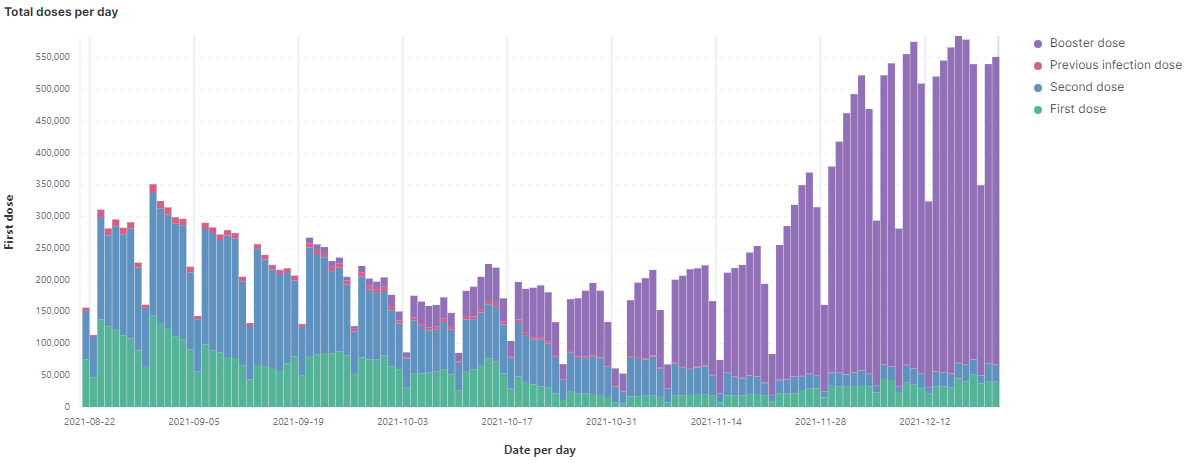
\includegraphics[width=\linewidth]{dashboards/dash1.png}
\end{figure}
\clearpage
\subsection{Total doses per region and provider in Italy}

\paragraph{}This representation is also derived from the second query and it shows for each vaccine provider the percentage of vaccinations for each region. We can focus on a specific region or a specific provider.\\
As we can see Astrazeneca in the last months has almost vanished, but if we extend the time horizon to the previous months the slice gets bigger
\begin{figure}[h]
	\centering
  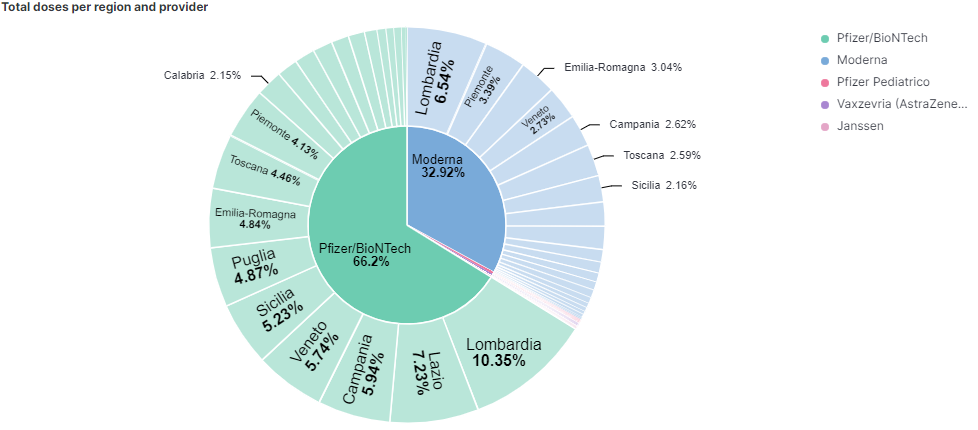
\includegraphics[width=\linewidth]{dashboards/dash2.png}
\end{figure}

\subsection{Total doses per age range and provider in Italy}

\paragraph{}This representation is derived from a generalization of the third query, it shows the total doses divided per age range and breaked down by vaccine type.
We can modify the time horizon as we please and focus on just a limited types of vaccinations or age ranges.\\
We can make the same conclusion about the Astrazeneca vaccine.
\begin{figure}[h]
	\centering
  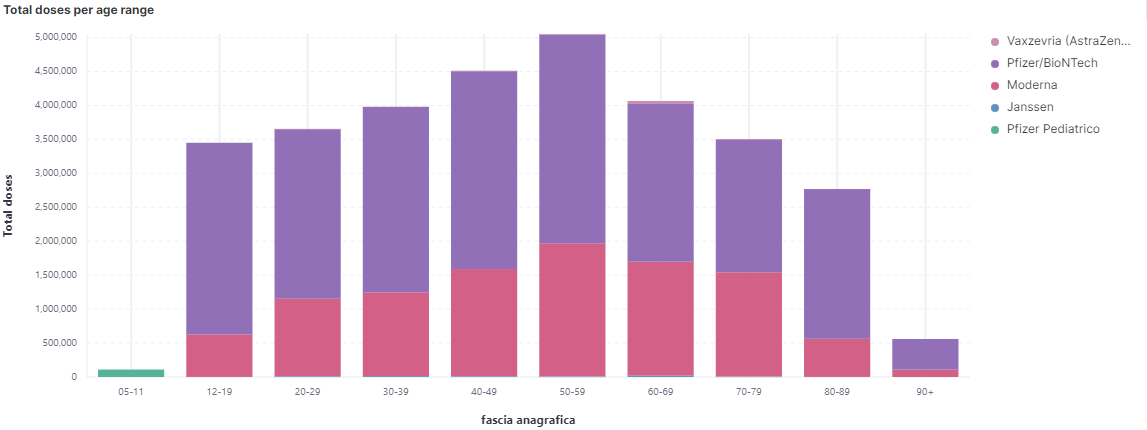
\includegraphics[width=\linewidth]{dashboards/dash3.png}
\end{figure}

\subsection{Gender comparison on total vaccinations in Italy}

\paragraph{}This representation shows the total vaccinations breaked down by vaccine type in percentage, between male and female. \\
We can focus on just one type of vaccine or gender.
\begin{figure}[h]
	\centering
  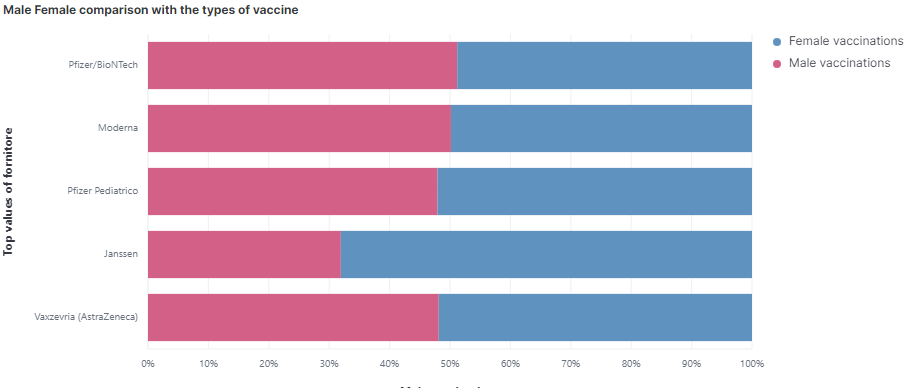
\includegraphics[width=\linewidth]{dashboards/dash4.png}
\end{figure}

\subsection{Trend of vaccines compared with deaths and infections in Italy}

\paragraph{}In this representation we mixed two different indexes ( vaccinations and global infections/deaths) in order to get a comparison of this data in Italy in the same graph.
\\
We can navigate the graph exploiting the informations of just one index for example hiding the information about the vaccinations to get a clearer graph about infections and deaths.
\begin{figure}[h]
	\centering
  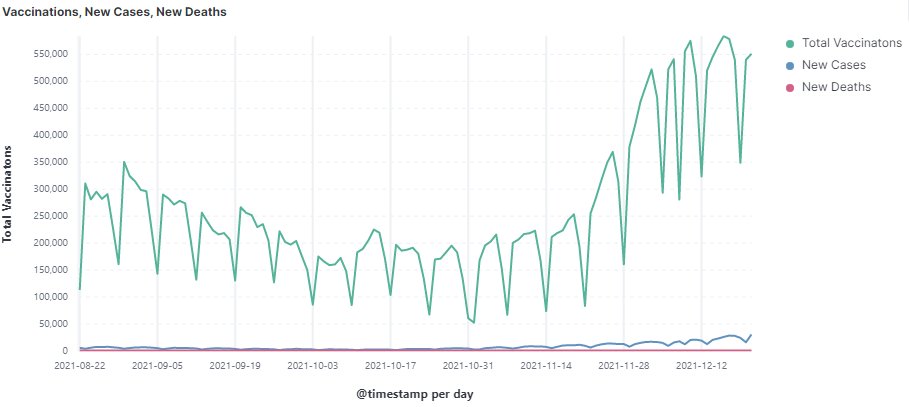
\includegraphics[width=\linewidth]{dashboards/dash5.png}
\end{figure}
\clearpage
\subsection{Trend of new cases in the world}

\paragraph{}In this representation we exploits the global index to get a trend of the continents new cases per million and we compare it with the new cases in Italy (red line).
\begin{figure}[h]
	\centering
  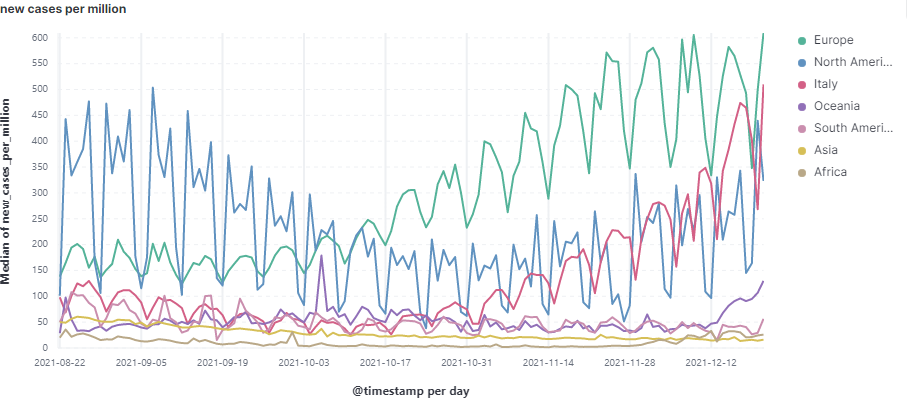
\includegraphics[width=\linewidth]{dashboards/dash6.png}
\end{figure}

\subsection{Trend of new cases in the italian regions}
\paragraph{}In this representation we exploits the regional infection index to get a trend of the italian regional new cases. \\ We can navigate the graph and select each region, or set of regions, one by one to get a clearer view of the trend.
\begin{figure}[h]
	\centering
  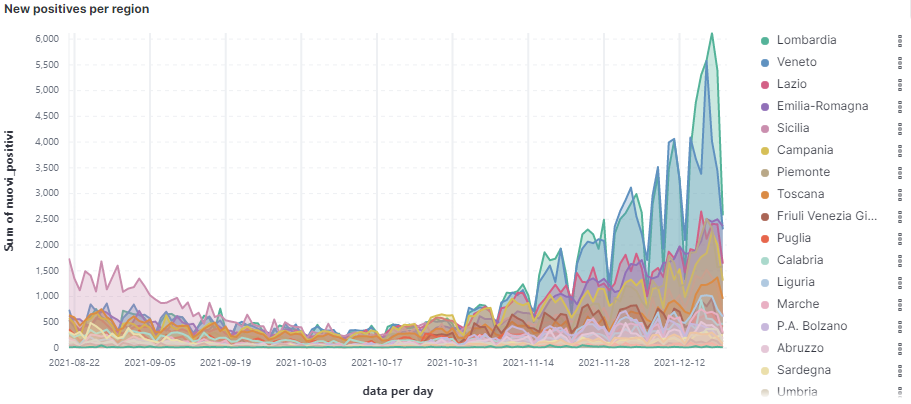
\includegraphics[width=\linewidth]{dashboards/dash7.png}
\end{figure}

\subsection{Trend of intensive care occupation and hospitalization in Italy}
\paragraph{}In this representation we exploits the regional infection index to get a trend of the hospitalization compared with the intensive care occupations. \\It is paramount important to keep checked this information in order to avoid health crisis.
\begin{figure}[h]
	\centering
  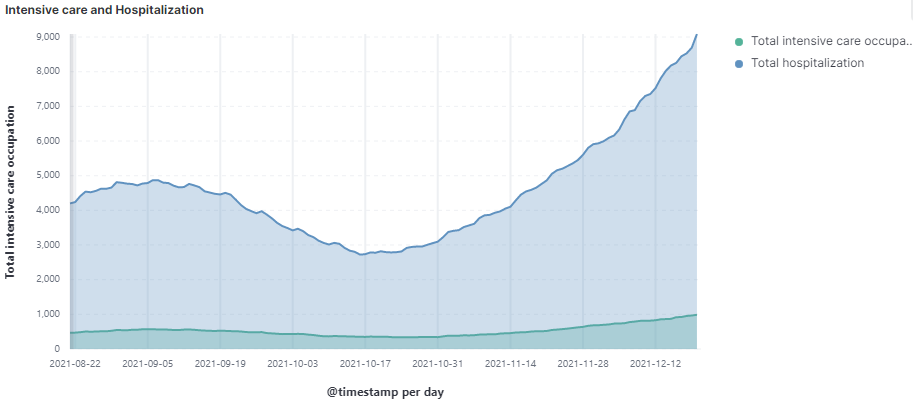
\includegraphics[width=\linewidth]{dashboards/dash8.png}
\end{figure}

\subsection{Mortality in the italian regions}
\paragraph{}In this representation we can compare the percentage mortality region by region.
It is interesting trying to understand the meaning behind this graph.
\begin{figure}[h]
	\centering
  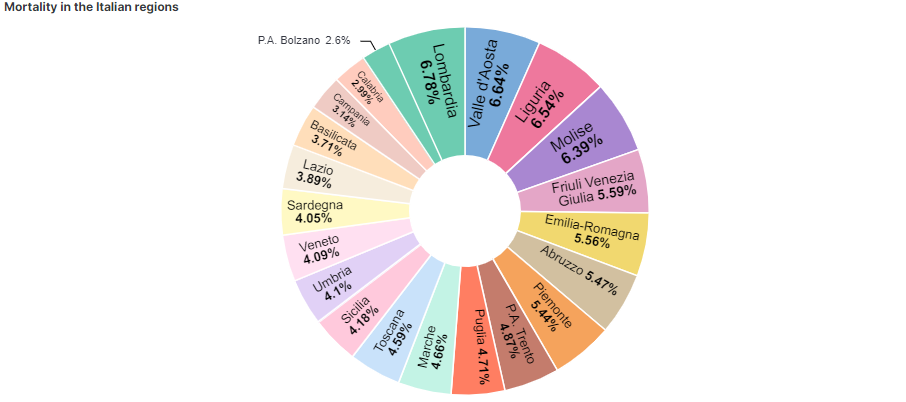
\includegraphics[width=\linewidth]{dashboards/dash9.png}
\end{figure}

\subsection{Variants percentage spread of variants in a given week}
\paragraph{}In this last representation we exploit the variants index in order to visualize the query number 8, that is, the spread on a pie chart of the variants in Italy the 32th week of the 2021.
\begin{figure}[h]
	\centering
  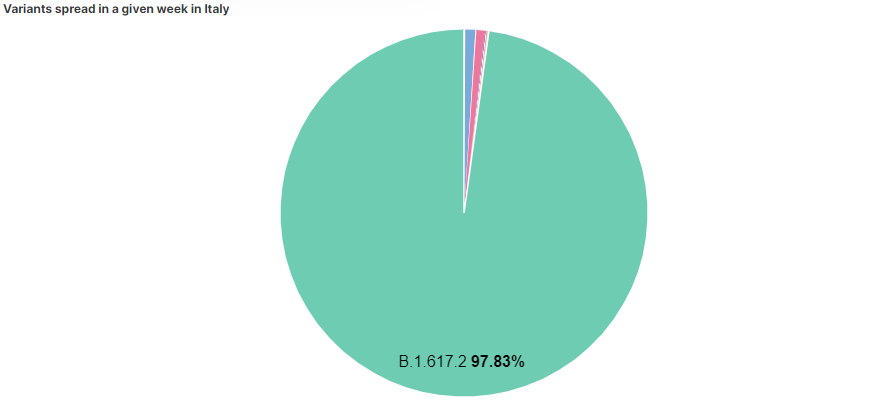
\includegraphics[width=\linewidth]{dashboards/dash10.png}
\end{figure}

\clearpage
\section{References \& Sources}
  \begin{thebibliography}{9}
    \bibitem{} Course Slides
    \bibitem{} https://pysimplegui.readthedocs.io/en/latest/call\%20reference/
    \bibitem{} https://docs.mongodb.com/manual/
    \bibitem{} https://pymongo.readthedocs.io/en/stable/
    \bibitem{} http://iniball.altervista.org/Software/ProgER
    \bibitem{} https://pandas.pydata.org/docs/
  \end{thebibliography}
\end{document}
